\chapter{实验测试与分析}
\label{sec:Experiment}

在本章中,将给出基于真实世界数据集的评估结果,以证明本文针对加密重复数据删除提出的频率分析攻击方法的有效性(对加密重复数据删除的威胁的严重性)。

\section{实验方法}
\label{sec:dataset}

本文所使用的真实世界数据集不包数据的实际内容,因此基于数据块哈希模拟攻击者所拥有的的对抗性知识。具体来说,本文将一些快照中的有序的数据块哈希列表作为辅助信息$\mathbf{A}$和原始明文信息$\mathbf{M}$。为了模拟加密过程,在$\mathbf{M}$中的每个原始数据块哈希(表示明文)上应用额外的哈希函数,并将结果截断为当前使用的数据集中约定的哈希值的长度。截断的结果用于模仿$\mathbf{C}$中的密文。对于每个推断的密文数据块-明文数据块对$(C,M)$,本文通过在$M$上应用相同的模拟加密并将结果与​​$C$进行比较来验证其正确性。特别的,基于聚类的频率分析攻击可以在数据段级别进行操作,断出密文数据段-明文数据段对$(S_\mathbf{C},S_\mathbf {A})$。在这种情况下,本文通过检查$S_\mathbf{C}$中的每个密文是否完全映射到$S_\mathbf{A}$中的每个明文来评估$(S_\mathbf {C},S_\mathbf{A})$的正确性。

本文通过推理率和推理精度两个标准来衡量攻击的有效性(参见\ref{sec:ThreatModel})。


\section{基于分布的攻击的实验结果}
\label{sec:experiment-distribution}

\subsection{实验1(参数的影响)}
\label{sec:exp1}

本节将评估参数$(u, r, t)$的变化在基于分布的频率分析攻击中带来的影响。实验使用FSL数据集(参见\ref{sec:fsl})来进行评估。在实验中使用每个用户的第12周备份作为辅助信息来推断该用户相应的第14周备份中的原始明文数据。出于控制变量的需求,实验将在固定另两个参数的前提下对三个参数中的一个的变化进行测试和分析。


\subsubsection{参数$u$的影响}

首先,配置参数$t \rightarrow \infty$和$r = 0$来评估参数$u$变化的影响(在这种情况下,基于分发的攻击将退化到基于数据块局部性的的攻击\cite{li2017information})。

\begin{figure}[!htbp]
    \centering
    \begin{tabular}{p{.48\linewidth}p{.48\linewidth}}
        \multicolumn{2}{c}{
\includegraphics[width=.7\textwidth]{legend-fsl-line.pdf}}  \\
        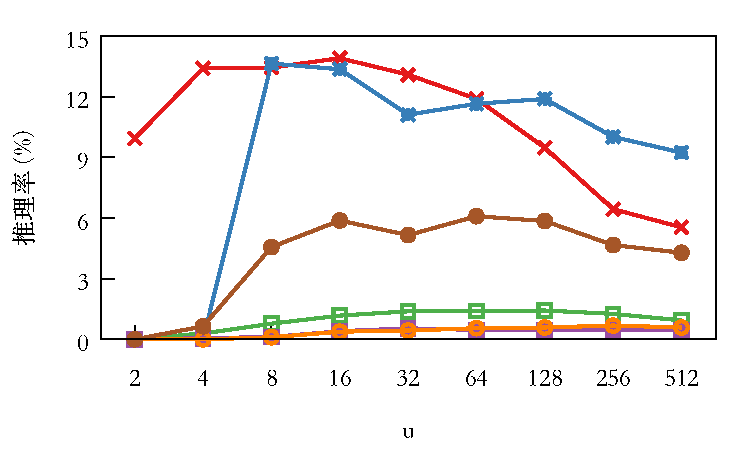
\includegraphics[width=\linewidth]{dis-impact-u-rate.pdf} &
        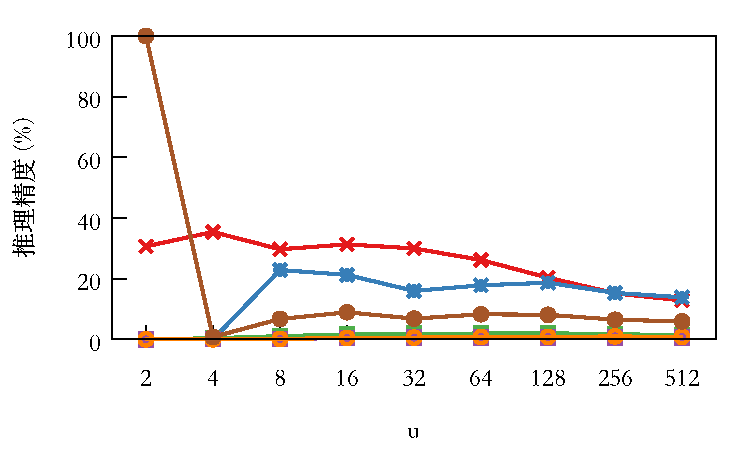
\includegraphics[width=\linewidth]{dis-impact-u-accuracy.pdf}\\
    \end{tabular}
    \caption{基于分布的攻击实验1:参数$u$的变化对推理结果的影响($r = 0$;$t \rightarrow \infty$)}
    \label{fig:distribution-impact-u}
\end{figure}

图\ref{fig:distribution-impact-u}显示了将参数$u$从2变为512时对推理率和推理精度带来的影响。对于推理率的结果,本实验的观察结果与已有的工作\cite{li2017information}相同。推理率首先随着$u$的增大而提高,这是因为频率分析攻击可以推断出更多的密文数据块-明文数据块对。推理率在达到最大值之后(例如,User004为13.9\%,User007为13.6\%,User012为1.4\%,User013为0.5\%,User015为0.7\%,User028为6.1\%)开始下降。其原因在于频率分析引入了大量的误报,这些误报会继续影响基于分布的攻击对每个数据块相邻邻居的推断。同时,部分特殊情况下的推理率约为0.0001\%,这意味着攻击只能推断出几个密文数据块-明文数据块对。

已有的工作\cite{li2017information}不提供基于数据块局部性的攻击的推理精度信息,因此本文提出的两种推理攻击方法的实验的推理精度的部分不与其进行对比。实验中观察到除User028的数据在$u=2$的条件下没有引入任何误报外,针对所有用户备份数据的推理精度都处于相当低的水平(小于40\%)。随着$u$的增大,推理精度会略有下降。例如,当$u$从2增加到512时,User004的推理精度从30.7\%下降到12.8\%。
    
\textbf{结论(1):}相对较大的$u$提高了推理率,但降低了推理精度(即,引入了更多的误报)


\subsubsection{参数$r$的影响}

然后,通过$u$变化的影响分析,本文选择增加推断的密文数据块-明文数据块对的覆盖范围,同时使用$r$和$t$来过滤可能的误报。因此,本文将User004,User013和User015的$u$设置为128,User007,User012和User028的设置分别为256,以评估$r$和$t$变化的影响。 

\begin{figure}[!htbp]
    \centering
    \begin{tabular}{p{.48\linewidth}p{.48\linewidth}}
        \multicolumn{2}{c}{
\includegraphics[width=.7\textwidth]{legend-fsl-line.pdf}}  \\
        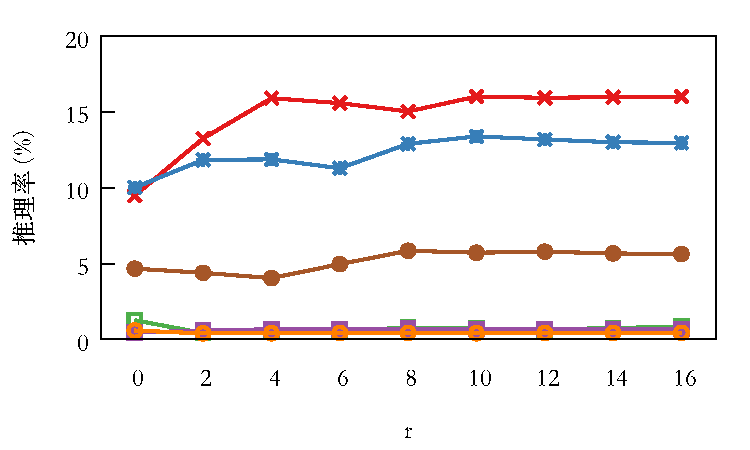
\includegraphics[width=\linewidth]{dis-impact-r-rate.pdf} &
        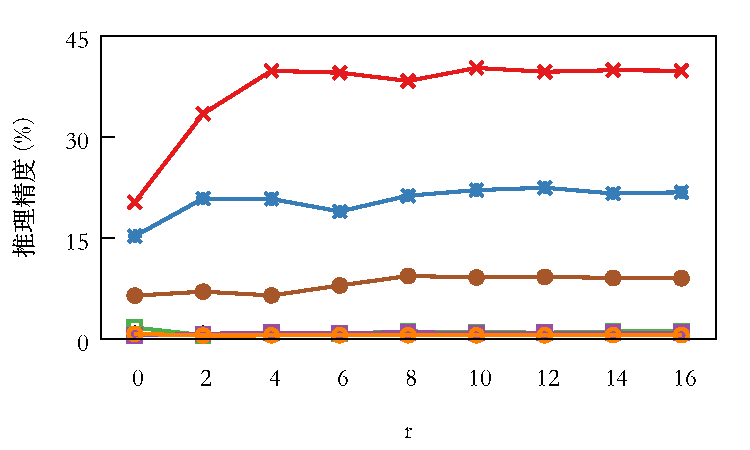
\includegraphics[width=\linewidth]{dis-impact-r-accuracy.pdf}\\
    \end{tabular}
    \caption{基于分布的攻击实验1:参数$r$的变化对推理结果的影响(User004、User013和User015中$u = 128$,User007、User012和User028中$u = 256$;$t \rightarrow \infty$)}
    \label{fig:distribution-impact-r}
\end{figure}

本实验中首先令$t\rightarrow \infty$,然后评估$r$变化带来的影响。图\ref{fig:distribution-impact-r}展示了参数$r$变化的实验结果。 实验观察到大多数用户的推理率随着$r$而增加。例如,当将$r$从0变为16时,User004推理率从9.5\%增加到16.0\%,User007从10.0\%增加到13.0\%,User013从0.5\%增加到0.7\%,User028从4.7\%增加到5.6\%。发生这种现象的原因是基于分布的攻击减少了直接频率排序的干扰,并推断出更多正确的密文数据块-明文数据块对。另一方面,对于User012和User015,推理率分别从1.3\%降至0.8\%,从0.6\%降至0.4\%。原因是随着检查的扩大,可能引入更多的误报。同时,所有用户的推断精度均处于低水平(小于45%),并且具有与其相应的推断率类似的变化趋势。


\textbf{结论(2):}较大的$r$提供了识别正确的密文数据块-明文数据块对的更多机会,但也增加了发生误报的概率。
\subsubsection{参数$t$的影响}

\begin{figure}[!ht]
    \centering
    \begin{tabular}{p{.48\linewidth}p{.48\linewidth}}
        \multicolumn{2}{c}{
\includegraphics[width=.7\textwidth]{legend-fsl-line.pdf}}  \\
        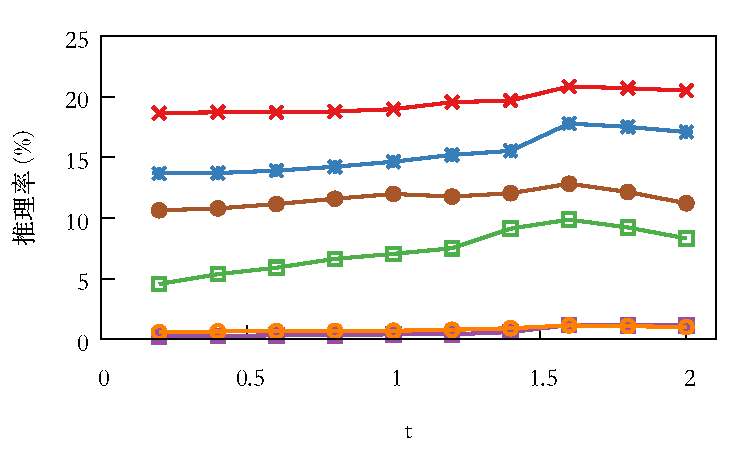
\includegraphics[width=\linewidth]{dis-impact-t-rate.pdf} &
        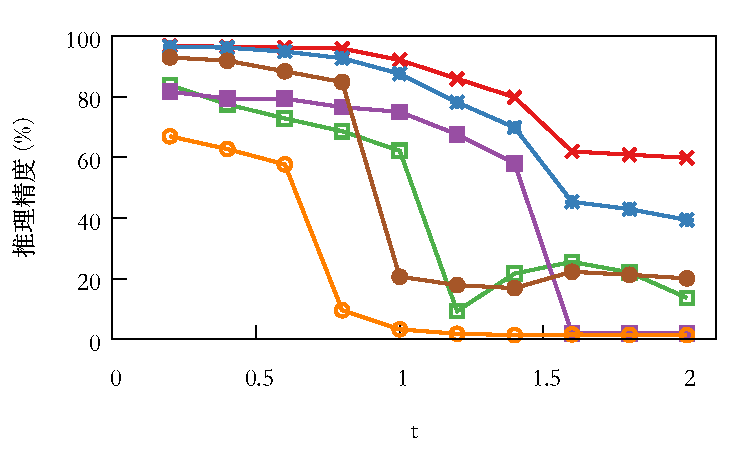
\includegraphics[width=\linewidth]{dis-impact-t-accuracy.pdf}\\
    \end{tabular}
    \caption{基于分布的攻击实验1:参数$t$的变化对推理结果的影响(User004、User013和User015中$u = 128$,User007、User012和User028中$u = 256$;$r = 10$)}
    \label{fig:distribution-impact-t}
\end{figure}

最后,设定$r=10$来评估参数$t$变化的影响。 图\ref{fig:distribution-impact-t}展示了参数$t$变化的实验结果果。当$t$很小(例如,小于0.5)时,实验观察到攻击误判并过滤了大量的密文数据块-明文数据块对,即使它们是正确的(即,引入了降低推理率的假阳性结果)。随着$t$的增加,假阳性的结果数量减少。当$t= 1.5$时,对于User004,User007,User012,User013,User015和User028,推理率分别达到最大值21.2\%,18.2\%,10.4\%,1.2\%,1.2\%和13.5\%。 当$t$进一步增大到2时,相应的推理率分别降至20.5\%,17.1\%,8.3\%,1.2\%,1.0\%和11.2\%。其原因是如果$t$过大,攻击就无法有效地过滤误报。因此,所有用户数据的推理精度都会随着$t$的增大而下降。

\textbf{结论(3):}较小的$t$过滤了大部分频率分析带来的误报,但它引入了更多的假阳性结果,导致了推理率的下降。

\subsection{实验2(与已有工作的对比)}
\label{sec:exp2}
本文将基于分布的攻击的有效性与基于数据块局部性的攻击的有效性进行比较\cite{li2017information}。除了使用实验1(参见\ref{sec:exp1})中采用的FSL数据集之外,本文还加入MS数据集(参见\ref{sec:ubc-ms})用于进行跨数据集的验证与评估。在MS数据集中,对于每个系统类别,一次选择两个快照,使用其中一个来推断另一个,以此评估平均的推理率和推理精度。

本文考虑采用以下攻击实例来进行比较。

\begin{itemize}[leftmargin=*]
\item \textbf{$\tt Baseline$:}

实验根据已有工作\cite{li2017information}中建议的参数配置实现基于数据块局部性的攻击。具体来说,它在频率分析的第一次调用中推断出5个出现频率最高的的密文数据块-明文数据块对(即,初始化一组用于迭代的密文数据块-明文数据块对),并且在每次后续调用中根据已有数据块对的邻居推断30个新的数据块对(即,迭代地推断密文数据块-明文数据块对)。

\item \textbf{$\tt Distribution$和$\tt Distribution^S$:} 

考虑两个基于分布的攻击的攻击实例,分别由$\tt Distribution$和$\tt Distribution^S$表示,它们分别使用和不使用大小信息作为辅助信息(即上标$\tt S$表示攻击实例使用大小信息进行操作)。实验在与${\tt Baseline}$相同参数的条件下配置$\tt Distribution^S$和${\tt Distribution}$。 此外,实验通过以下方式在$\tt Distribution^S$和${\tt Distribution}$中选择参数$r$和$t$的取值:对于FSL数据集,我们为所有用户设定$r = 10$,并分别为User004、User007、User012、User013、User015和User028设置参数$t$ = 1.5、1.2、1、1、0.7和0.9;对于MS数据集,实验继续为所有类别设置参数$r = 10$,为Win7和Serv-08设置参数$t = 2$,为Vista-U、Serv-03和Vista-B设置参数$t = 1.6$。以上数据是通过按照实验1(参见\ref{sec:exp1})的方法对数据集的最佳配置的测试得出的。 
\item \textbf{$\tt Distribution$-$\tt o$和$\tt Distribution^S$-$\tt o$:}

实验考虑另外两个基于分布的攻击的实例,用$\tt Distribution$-$\tt o$和$\tt Distribution^S$-$\tt o$表示,对于$r$和$t$应用与$\tt Distribution$和$\tt Distribution^S$相同的配置,但进一步使用更大的参数$u$增加推断的密文数据块-明文数据块对的覆盖范围。具体来说,实验通过以下方式在$\tt Distribution$-$\tt o$和$\tt Distribution^S$-$\tt o$中配置参数$u$:对于FSL数据集,参数$u$的选择与实验1(参见\ref{sec:exp1})相同;对于MS数据集,实验为Win7数据设置$u = 128$,为Serv-03、Serv-08、Vista-B和Vista-U设置$u  = 30$。 
\end{itemize}

\begin{figure*}[!htbp]
    \centering
    \begin{tabular}{c}
        
\includegraphics[width=.7\textwidth]{pic/legend-fsl-bar.pdf}\\
        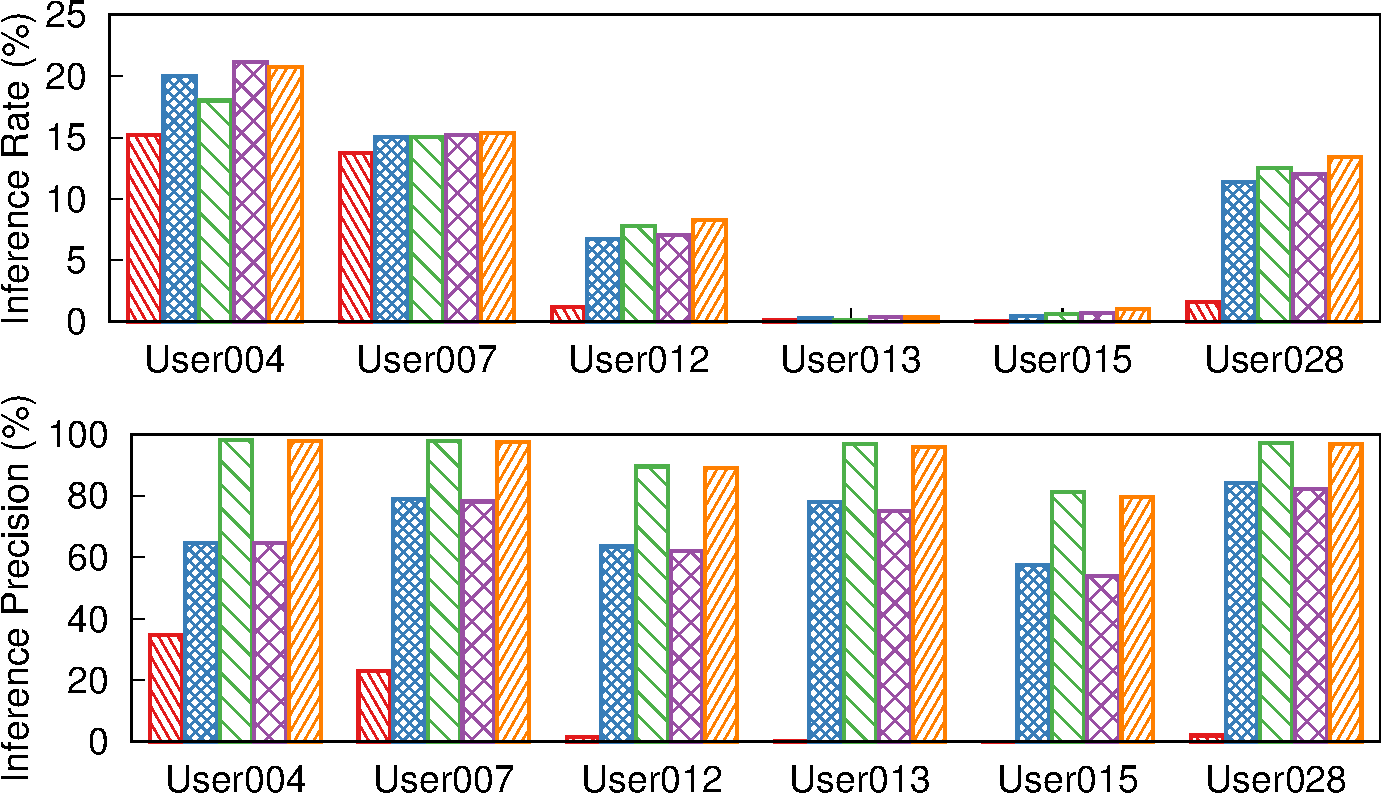
\includegraphics[width=.7\textwidth]{pic/distribution-comparison-fsl.pdf} 
    \end{tabular}
    \caption{基于分布的攻击实验2(与已有工作的对比):比较基于分布的攻击和基于数据块局部性的攻击的有效性(FSL数据集)。}
    \label{fig:distribution-comparison-fsl}
\end{figure*}

图\ref{fig:distribution-comparison-fsl}给出了基于FSL数据集的上述5种实例的比较结果。实验观察到,在几乎所有情况下,基于分布的攻击的不同实例都优于基于数据块局部性的攻击。例如,对于User028,基于分布的攻击的最低推理率是11.4\%,推理精度为84.1\%($\tt Distribution$);此时$\tt Baseline$相应的推理率仅为1.2\%,推理精度仅为1.7\%。这意味着在这种情况下,基于分布的攻击可以将假阳性的数量减少82.4\%。

\textbf{结论(4):}基于分布的攻击显着提高了推理精度,同时实现了比基于数据块局部性的攻击更高的推理率。 

$\tt Distribution^S$和$\tt Distribution^S$-$\tt o$相较于$\tt Distribution$和$\tt Distribution$-$\tt o$拥有更高的推理精度,这因为它们进一步通过数据块大小信息过滤了误报。例如,对于User004,$\tt Distribution^S$和$\tt Distribution^S$-$\tt o$相较于$\tt Distribution$和$\tt Distribution$-$\tt o$将误报分别从35.2\%减少到1.7\%,从35.3\%减少到2.2\%。然而,在同样的情况下,实验观察到$\tt Distribution$ and $\tt Distribution$-$\tt o$的推理率分别为20.0\%和21.2\%,相较于$\tt Distribution^S$和$\tt Distribution^S$-$\tt o$分别高出2.0\%和0.4\%。其原因是$\tt Distribution$和$\tt Distribution$-$\tt o$推断出了来自不正确的密文数据块-明文数据块对的邻居中的少量正确结果。换句话说,虽然$(C, M)$是不正确的密文数据块-明文数据块对,但$C$的邻居可能以很小的概率对应于$M$的邻居。即使在这种情况下,所有基于分布的攻击实例都比基于数据块局部性的攻击实例效果更佳。具体来说,$\tt Baseline$的推理率仅为15.2\%,比基于分布的攻击的最佳情况低6.0\%,最差情况低2.8\%。  

\textbf{结论(5):}过滤不正确的推理结果可以提高推理精度,但会降低推理的密文数据块-明文数据块对的覆盖范围,并可能降低推理率。

我们进一步观察到,虽然$\tt Distribution$-$\tt o$和$\tt Distribution^S$-$\tt o$构建在更大的参数$u$上,但它们的推理率仅略高于$\tt Distribution$和$\tt Distribution^S$(分别高为0.4\%和0.9\%)。 原因是基于分布的攻击仅通过已推理出数据块对的邻居进行迭代推理。参数$u$的进一步增大只会在结果中添加少量新的正确密文数据块-明文数据块对。

\begin{figure*}[t]
    \centering
    \begin{tabular}{c}
        
\includegraphics[width=.7\textwidth]{pic/legend-fsl-bar.pdf}\\
        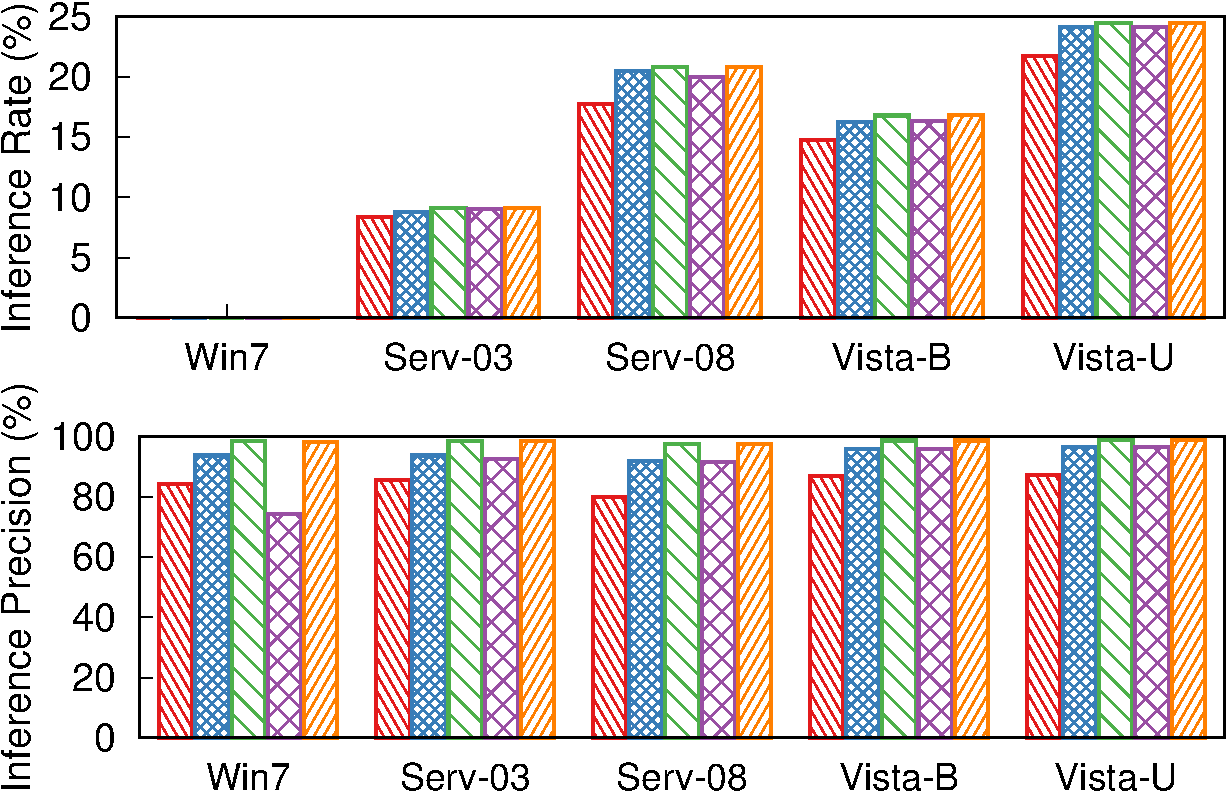
\includegraphics[width=.7\textwidth]{pic/distribution-comparison-ms.pdf}\\
    \end{tabular}
    \caption{基于分布的攻击实验2(与已有工作的对比):比较基于分布的攻击和基于数据块局部性的攻击的有效性(MS数据集)。}
    \label{fig:distribution-comparison-ms}
\end{figure*}


图\ref{fig:distribution-comparison-ms}给出了基于MS数据集的上述5种实例的比较结果。基于数据块局部性的攻击和基于分布的攻击在大多数MS数据集的类别(Win7除外)中具有高推理率和精度。可能的原因是MS数据集中的快照高度相关(例如,数据块总数的方差很小,如表\ref{tab:MS-dataset}所示)。实验观察到基于分布的攻击仍然优于基于数据块局部性的攻击。例如,在Vista-U中,基于分布的攻击的所有推理的推理率和推理精度分别高于24.1\%和96.4\%,而$\tt Baseline$的推断率和分辨率分别为21.7\%和87.1\%。

实验中对于数据集中Win7类别,基于分布的攻击和基于数据块局部性的攻击的推断率都很低(小于0.01%)。其原因是Win7包含大量具有唯一性的数据块(大约超过98.8\%,如表\ref{tab:MS-dataset}所示),导致了攻击效果表现不佳。

\subsection{实验3(攻击效果)} 

实验考虑长期备份模式,并使用FSL数据集检查基于分布的攻击的有效性。具体来说,实验选择每个用户的第$i$个FSL每周备份作为辅助信息,以推断相应的第$(i+w)$个FSL每周备份中的原始明文。显然,$w$越小,辅助信息和目标备份之间的相关性就越高。与实验2(参见\ref{sec:exp2})配置两个基于分布的攻击实例$\tt Distribution$-$\tt o$和$\tt Distribution^S$-$\tt o$,并评估它们的推理率和推理精度(针对每个用户的所有可用的$i$)。

\begin{figure*}[!htbp]
    \centering
    \centering
    \begin{tabular}{c}
        
\includegraphics[width=.35\textwidth]{legend-effectiveness.pdf}\\
        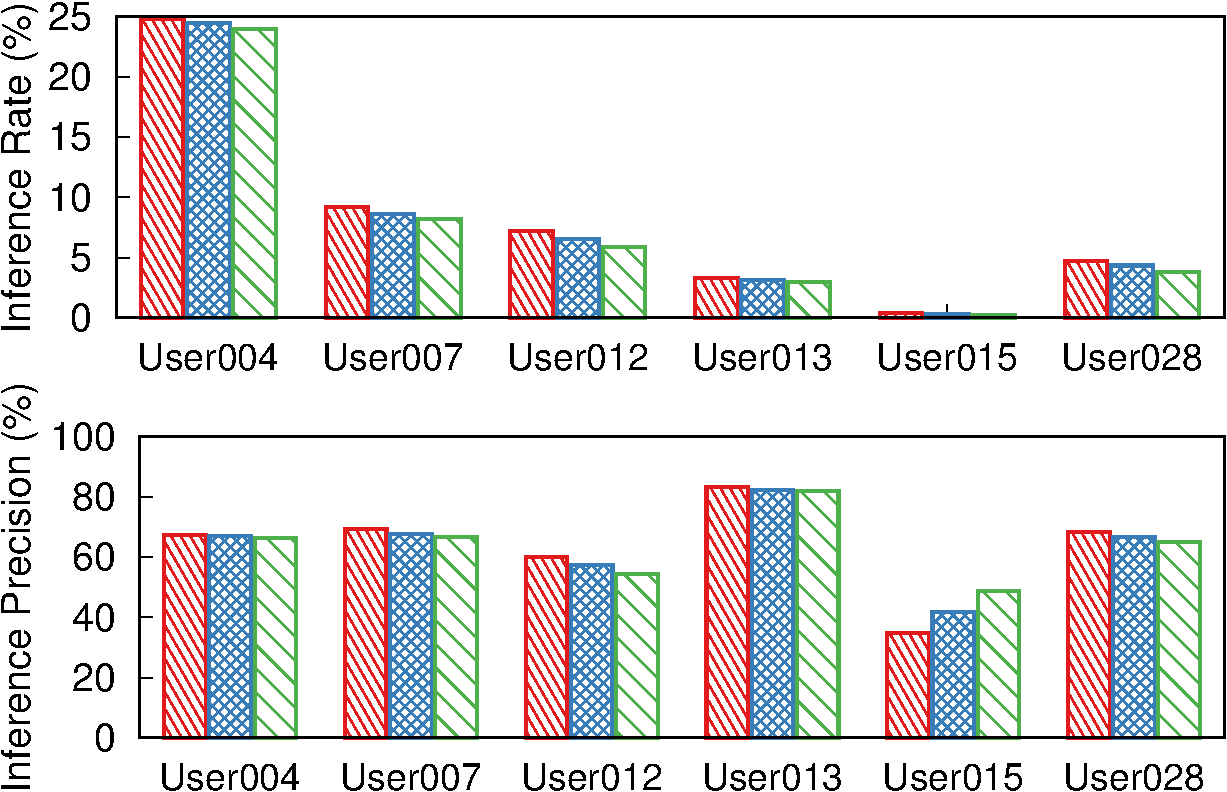
\includegraphics[width=.7\textwidth]{distribution-effectiveness-wo-size.pdf}
    \end{tabular}
	\caption{实验3(攻击效果):没有大小信息辅助的基于分布的攻击在FSL数据集中的有效性。}
	\label{fig:experiment-distribution-effectiveness-wo}
\end{figure*}

图\ref{fig:experiment-distribution-effectiveness-wo}给出了$\tt Distribution$-$\tt o$的实验结果。基于分布的攻击在用户之间具有不同的推理率和推理精度。例如,在类似User004这样的有利情况下,它实现了推理率24.8\%、推理精度67.3\%($w = 1$);推理率24.5\%、推理精度67.0\%($w = 2$);推理率24.0\%、推理精度66.5\%($w = 3$)。在类似User015这样的非有利情况下,基于分布的攻击的推理率仅有0.3\%。可能的原因是User015的备份数据具有较低的数据块局部性。

此外,实验观察到辅助信息的相关性(即$w$)对基于分布的攻击的有效性影响较低。例如,当$w$从1增加到3时,它仅导致推理率(下降小于1.4\%)和精度(下降小于5.6\%)的有限下降。其原因是基于分布的攻击解决了频率排名中的干扰并保留了攻击的有效性。

\textbf{结论(6):}基于分布的攻击可以在存在松散相关的辅助信息的帮助下有效控制攻击有效性的下降程度。

\begin{figure*}[!htbp]
    \centering
    \centering
    \begin{tabular}{c}
        
\includegraphics[width=.35\textwidth]{pic/legend-effectiveness.pdf}\\
        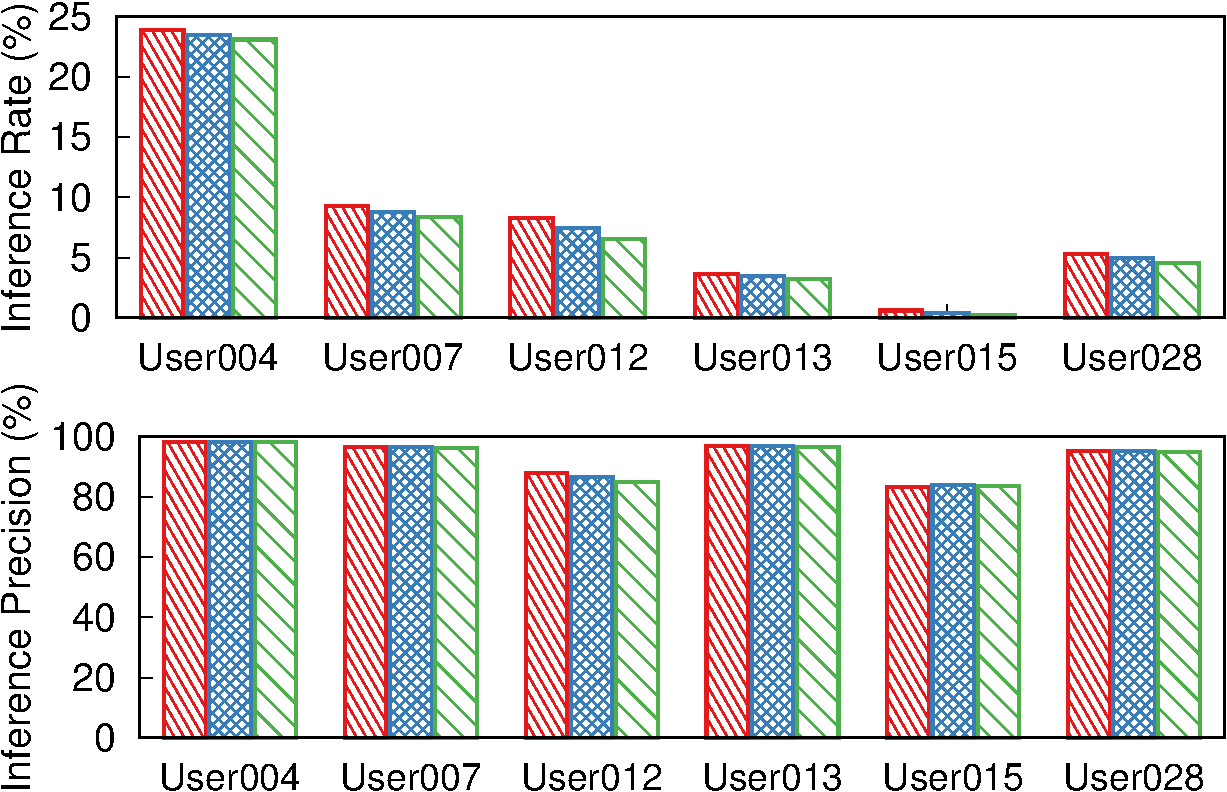
\includegraphics[width=.7\textwidth]{pic/distribution-effectiveness-w-size.pdf}
    \end{tabular}
	\caption{实验3(攻击效果):有大小信息辅助的基于分布的攻击在FSL数据集中的有效性。}
	\label{fig:experiment-distribution-effectiveness-w}
\end{figure*}

图\ref{fig:experiment-distribution-effectiveness-w}给出了$\tt Distribution^S$-$\tt o$的实验结果。实验观察到它具有与$\tt Distribution$-$\tt o$相似的推理率,同时拥有更高的推理精度。例如,对于所有用户的平均推断精度分别为93.1\%($w = 1$)、92.8\%($w = 2$)和92.4\%($w = 3$)。         

\section{基于聚类的攻击的实验结果}
\label{sec:experiment-clustering}

\subsection{实验4(参数的影响)} 

实验首先评估参数$k$的影响,该参数定义了凝聚法层次聚类中组合两个最近聚类的距离上限。本实验使用FSL和VM数据集来研究$k$如何影响攻击中的基础聚类方案。具体来说,分别对每个选出的FSL和VM用户数据的最后一次备份应用分段方法,并生成固定大小为4MB的数据段。

聚类方案旨在将类似的密文数据段聚合到同一个聚类中,这一过程不会损害每个密文数据段中的数据块的机密性。为了量化其影响,将聚类的结果与实际分类方法的结果进行比较(实际分类方法通过最小数据块哈希直接对分段进行分类)。假设我们分别通过实际分类方法生成$m$个数据段的集合,并且通过聚类方案生成$\widetilde{m}$个数据段的集合。通过$\frac{{\sf abs}(m-\widetilde{m})}{m}$(其中${\sf abs}(m-\widetilde{m})$返回$m-\widetilde{m}$的绝对值)衡量聚类形成的集合与实际分类形成的集合的相似程度。记集合所有数据段都相同(具有相同的最小数据块哈希)的聚类的数量为$\hat{m}$。此外,实验还考虑了聚类正确性,由$\frac{\hat{m}}{\widetilde{m}}$进行评估,它量化了对相似数据段的聚类方案的精确程度。


Figure~7(a) shows the results of the FSL dataset, where we consider four FSL users (e.g., User004, User007, User015 and User028) for saving evaluation time. The clustering closeness first increases with $k$, since the number (i.e., $\widetilde{m}$) of clusters decreases and approximates $m$. When $k$ increases further, the number of clusters drops away from $m$, and leads to the increase of clustering closeness.  In addition, we observe that the clustering correctness gradually decreases with $k$, because some of non-similar segments (i.e., their minimum chunk hashes are different) are aggregated into the same cluster. Both results suggest that we can configure an appropriate $k$ to balance the closeness and correctness of clustering. For example, when we set $k$ = 0.65 for User015, the corresponding closeness and correctness are 1.0\% and 94.2\%, respectively. This implies that the results of the clustering scheme  highly approximates those of real classification.             

{\bf Observation (7) --} {\em By configuring an appropriate $k$ for clustering, we  approximate the results of  classifying segments, without the knowledge of  minimum chunk hash in each segment.}   

Figure~7(b) shows the results of the VM dataset. We observe that the clustering closeness and correctness of all VM users have  similar tendencies with those of FSL users. When we configure $k$ = 0.8, the average clustering closeness of all VM users is only 3.0\%, while the corresponding clustering correctness is as high as 93.1\%.     


\begin{figure*}[!htbp]
\centering
    \begin{tabular}{cc@{\hspace{0.3in}}p{.32\textwidth}}
    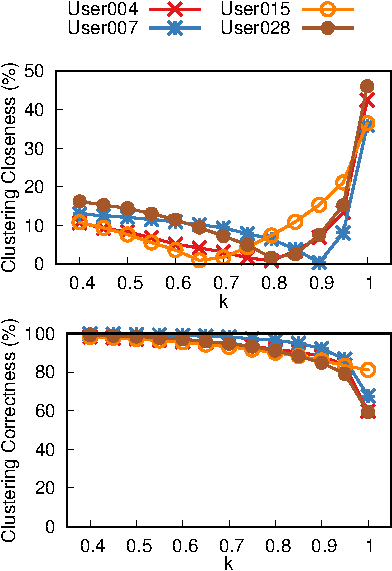
\includegraphics[width=.3\textwidth]{pic/clustering-impact-d-fsl.pdf} &
    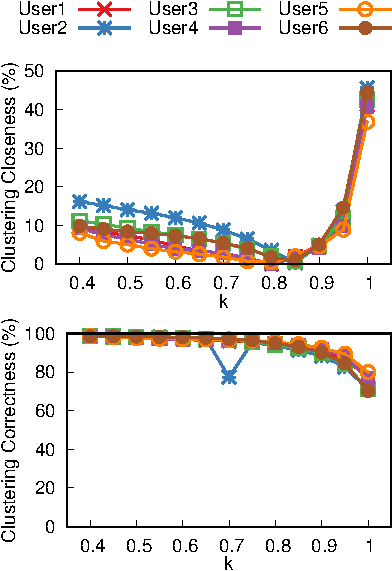
\includegraphics[width=.3\textwidth]{pic/clustering-impact-d-vm.pdf} & 
    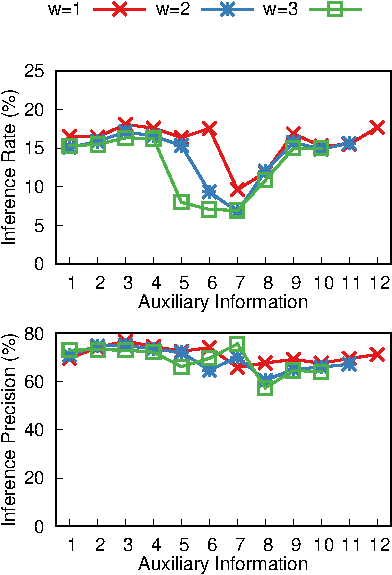
\includegraphics[width=.3\textwidth]{pic/clustering-effectiveness.pdf} \medskip \\
{\footnotesize 
        (a) FSL dataset } 
&
{\footnotesize 
        (a) VM dataset } 
        &  ~~~ \medskip \\
        \multicolumn{2}{p{.64\textwidth}}{
            \footnotesize Fig.~7\quad Experiment 4 (Impact of parameter): impact of $k$ in the clustering scheme; for clustering closeness, the smaller the better; for clustering correctness, the larger the better. } &
        {\footnotesize
Fig.~8\quad Experiment 5 (Attack effectiveness):  severity of clustering-based attack in VM dataset.
        }
\end{tabular}
    \hspace{-1in}
\end{figure*}


\begin{table*}[!htbp]
\small
    \caption{Experiment 6 (Security implications)}
\renewcommand{\arraystretch}{1.2}
\vspace{-3pt}
 \begin{minipage}[t]{0.7\textwidth}
\centering
        (a) Distribution-based attacks \medskip \\
\begin{tabular}{|c|c|c|c|c|c|}
\hline

    \multirow{2}{*}{\bf Type} & \multirow{2}{*}{\bf Extension Name} & \multirow{2}{*}{\bf \centering Range of File Size}  & \multicolumn{2}{c|}{\bf Raw Inference Rate} \\ \cline{4-5} 
    & & &  $\sf Distribution$-$\sf o$ & $\sf Distribution^S$-$\sf o$ \\ \hline
\hline
    Office & doc(x), ppt(x), xls(x) & 10KB-1MB   & 4.9\% & 5.3\%\\
\hline
    Picture & jpg, png &10-100KB  & 7.7\% & 6.7\% \\
\hline
    Source & c, h, cpp, java, py & 10-20KB   & 17.1\% & 15.0\%\\
\hline
    Database & db, po & 20-700KB   & 2.6\% & 2.4\%\\
\hline
    Disk & vmdk, img & 200MB-1GB  & 15.8\% & 16.7\%\\
\hline
\end{tabular}
\label{tab:file}
 \end{minipage}
\hfill
    \begin{minipage}[t]{0.3\textwidth}
    \centering
        (b) Clustering-based attack \medskip \\
    \begin{tabular}{|c|c|}
    \hline
        {\bf Users} & {\bf Raw Inference Rate} \\
    \hline
    \hline
        1 & 13.2\% \\ 
    \hline
        2 & 22.4\% \\ 
    \hline
        3 & 25.7\% \\ 
    \hline
        4 & 28.4\% \\ 
    \hline
        5 & 18.5\% \\ 
    \hline
        6 & 30.8\% \\ 
    \hline
    \end{tabular}
\label{tab:user}
    \end{minipage}

\end{table*}



\subsection{实验5(攻击效果)} 

We now study the
effectiveness of the clustering-based attack. Due to the boundary shift of
fixed-size segment, it has low effectiveness
(about 1\% inference rate in our test) against the FSL dataset.  Thus, we use
the VM dataset to examine its severity. To configure the attack, we set $k$ =
0.8 for clustering, and $(u, r, t)$ = (5000, 100, 0.5) for relating ciphertext
clusters to corresponding plaintext clusters.  

In our micro-benchmarking, we find that the chunk-level inference in the
clustering-based attack only infers thousands of chunks correctly, which
contributes to a negligible inference rate (e.g., less than 0.01\%).  
% The
% reason is that each cluster includes a large number of chunks, and frequency
% analysis is ineffective in this case. 
Thus, we focus on the
segment-level inference, which presents the bottom line of severity in the
clustering-based attack. To be consistent with the chunk-level measurements, we count inference rate and precision based
on the unique chunks in each correctly inferred segment. 

We use the same evaluation methodology of Experiment~3, and report the results
in Figure~8. Specifically, the x-axis describes the index $i$ (where 1 $\leq i \leq$
12) of the VM backup that is used as the auxiliary information for attack,
while the y-axis presents the average inference rate or precision of all VM
users against the $(i+w)$th backup (where $w$ = 1, 2, and 3). We observe that both the inference rate and the inference
precision fluctuate significantly. For example, when using the 3rd backup as
the auxiliary information, the attack achieves the highest inference rates at
18.1\%, 17.1\% and 16.3\%, with the precisions of 76.8\%, 75.0\% and 73.0\%
for $w$ = 1, 2, and 3, respectively. 
On the other hand, when using the 7th
backup as the auxiliary information, the corresponding inference rates and
precisions drop down to 9.6\% and 65.9\%, 6.8\% and 71.2\%, and 6.9\% and
75.6\%, respectively. The reason is that the VM users have heavy updates after
the 7th week, and this reduces the correlation  of adjacent backups. 
On
average, for $w$ = 1, 2 and 3, the clustering-based attack infers 15.8\%,
14.0\%, and 12.6\% ciphertext-plaintext pairs, with the precisions of 71.1\%,
69.1\%, and 68.9\%, respectively. 
% This demonstrates high severity against
% the VM disk images.   

\section{攻击对安全影响的结果}
\label{sec:case}

We thus far have examined the severity of inference attacks by quantifying the correctly inferred ciphertext-plaintext pairs.  However, it remains an open issue that what are the security implications informed by these results and how the frequency analysis attacks bring actual damage. In the following experiment, we evaluate the security implications of our attacks based on the raw inference rate, defined as the percentage of raw data content affected by correctly inferred chunks.   




\subsection{实验6(安全隐患分析)}

We first consider the distribution-based attack, and evaluate its raw
inference rate against {\em different types} of files. We drive the evaluation
using the FSL dataset, since only the FSL dataset includes file metadata (that
includes the extension names of files) in plaintext. Specifically, we focus on
five types of files that have specific extension names (see
Table~\ref{tab:file}(a)): office files ({\em Office}), picture files 
({\em Picture}), programming source files ({\em Source}), database files 
({\em Database}), and disk image files ({\em Disk}). These files occupy more
than 60\% of raw content of FSL snapshots.   

We apply the methodology of Experiment~2, and evaluate the raw inference
rates of $\sf Distribution^S$-$\sf o$ and $\sf Distribution$-$\sf o$. 
Table~\ref{tab:file}(a) shows the results. Both attack instances have high raw
inference rates against {\em Disk} (e.g., 15.8\% for 
$\sf Distribution$-$\sf o$ and 16.7\% for $\sf Distribution^S$-$\sf o$),
because each disk file includes a large number of rarely updated chunks that
form high locality within the same file. Interestingly, we observe that 
{\em Source}, although each file is of a small size, also incurs high raw
inference rates by the distribution-based attacks (e.g., 17.1\% for 
$\sf Distribution$-$\sf o$ and 15.0\% for $\sf Distribution^S$-$\sf o$). The
reason is that programming source files are often stored together in file system
(e.g., the source files that belong to the same project locate in an identical
directory) and form a large stretch of correlated chunks, which present high
locality across files. For small and scattered files (e.g., {\em Office}, 
{\em Picture}, and {\em Database}), the distribution-based attacks have
relative low raw inference rates.     


{\bf Observation (8) --} {\em The severity of the distribution-based attack depends on the update frequencies, sizes, and spatiality of target files. } 

We examine the security implication of the clustering-based attack using the VM dataset. Specifically, we use the 11th  backup of each VM user  to infer original content in corresponding 13th VM backup. Since the VM dataset does not contain any metadata, we count the raw inference rate based on the  whole data content in each VM snapshot. Note that we filter all zero chunks in the count of raw inference rate, because they occupy a large fraction in VM disk images \cite{jin09}.           

We use the same configuration of Experiment~5, and evaluate raw inference rate
based on segment-level inference.  Table~\ref{tab:user}(b) shows the results
for different users.  We observe that the clustering-based attack achieves high
severity against the VM dataset. For example, it infers up to 30.8\% raw
content of User6's VM backup. On average, the raw inference rate of all users
is as high as 23.2\%.  

{\bf Observation (9) --} {\em The clustering-based attack threatens the
confidentiality of VM disk images. } 

\section{本章小结}

